Este trabajo consiste en implementar filtros gráficos utilizando el modelo de procesamiento SIMD. De esta manera procesaremos, por ejemplo, 4 píxeles de una imagen al mismo tiempo. Se busca encontrar una mejora significativa entre la utilización de dichos registros $XMM$ contra el proceso provisto en el lenguaje de programación $C$. 

% Esta parte no me cierra, la puedo mejorar.
Se abarcaran 4 conocidos filtros de imágenes distintos provistos por la cátedra. Estos filtros son:

\subsection{Tres Colores}

Este filtro realiza un cambio en los colores de cada pixel en base a 3 colores fijos que son: 

\begin{itemize}
  \item Crema (R: 236, G: 233, B: 214)
  \item Verde (R: 0, G: 112, B: 110)
  \item Rojo (R: 244, G: 88, B: 65)
\end{itemize}

Una vez definidos los 3 colores, utilizaremos el brillo que equivale a la suma de los 3 colores de cada píxel dividido 3. Este mismo brillo con distintas comparaciones nos indica como reformular el nuevo color que utilizaremos.

Con lo que obtendremos imagenes como esta:

\begin{figure}[H]
    \centering
    \begin{subfigure}[H]{0.5\textwidth}
        \centering
        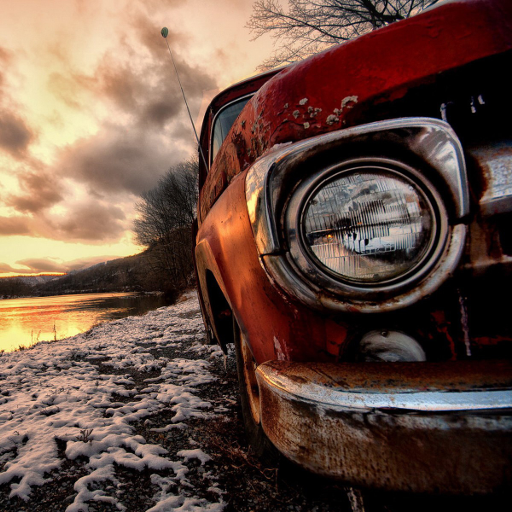
\includegraphics[width=7cm, height=6cm]{images/car.png}
        \caption{Original}
    \end{subfigure}%
    ~ 
    \begin{subfigure}[H]{0.5\textwidth}
        \centering
        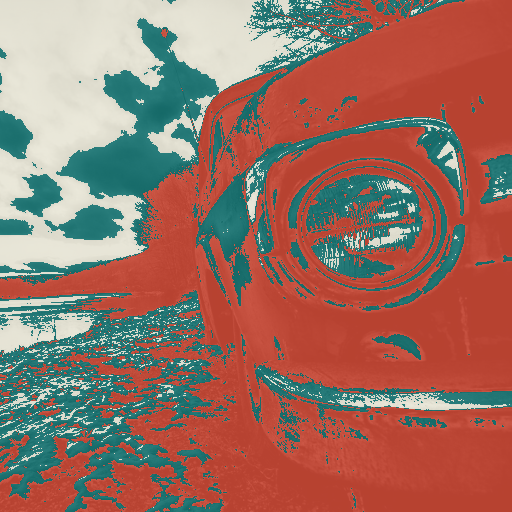
\includegraphics[width=7cm, height=6cm]{images/img_tresColores.png}
        \caption{Con Tres Colores}
    \end{subfigure}
    \caption{Caption place holder}
\end{figure} 


\subsection{Efecto Bayer}

Este filtro elimina 2 de los 3 colores de cada píxel dejando únicamente el color marcado en la siguiente ilustración:

\begin{table}[h]
\begin{center}
\begin{tabular}{|c|c|c|c|c|}
\hline
 Rojo     & Verde \\ \hline
 Verde    & Azul \\ \hline
\end{tabular}
\end{center}
\end{table}

Expandiendo este mismo patrón desde la esquina superior izquierda a la esquina inferior derecha. 

Por ejemplo:

\begin{figure}[H]
    \centering
    \begin{subfigure}[H]{0.5\textwidth}
        \centering
        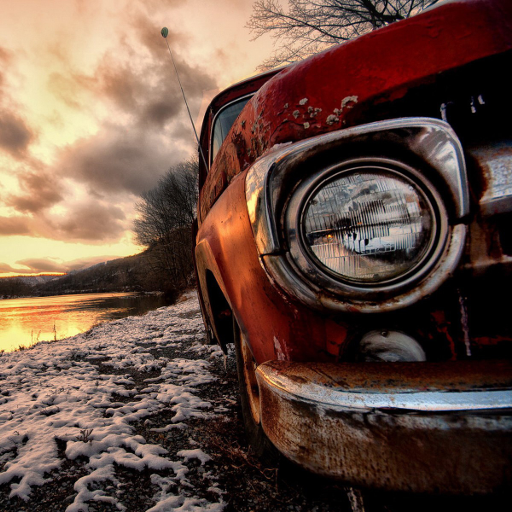
\includegraphics[width=7cm, height=6cm]{images/car.png}
        \caption{Original}
    \end{subfigure}%
    ~ 
    \begin{subfigure}[H]{0.5\textwidth}
        \centering
        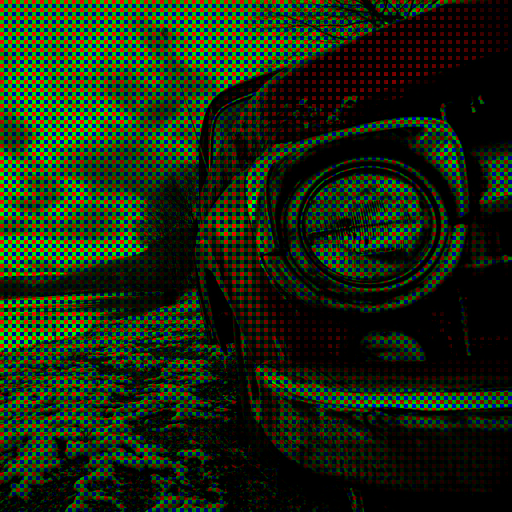
\includegraphics[width=7cm, height=6cm]{images/img_efectoBayer.png}
        \caption{Con Efecto Bayer}
    \end{subfigure}
    \caption{Caption place holder}
\end{figure} 

\subsection{Cambia Color}

Sobre este filtro hay 2 posibles escenarios para cada píxel, dependiendo de la distancia entre el píxel original y los parámetros de entrada se puede o no, cambiar el color del mismo. En la siguiente imagen veremos como sucede.

\begin{figure}[H]
    \centering
    \begin{subfigure}[H]{0.5\textwidth}
        \centering
        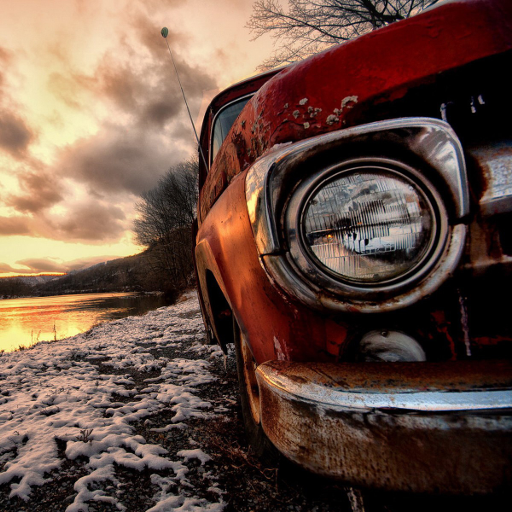
\includegraphics[width=7cm, height=6cm]{images/car.png}
        \caption{Original}
    \end{subfigure}%
    ~ 
    \begin{subfigure}[H]{0.5\textwidth}
        \centering
        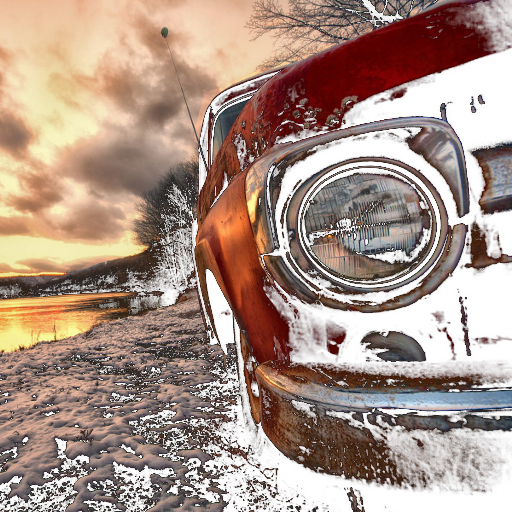
\includegraphics[width=7cm, height=6cm]{images/img_cambiaColor.png}
        \caption{Con Efecto Bayer}
    \end{subfigure}
    \caption{Caption place holder}
\end{figure} 


\subsection{Edge Sobel}

El filtro de $Edge$ $Sobel$ hace distintas operaciones utilizando solamente escala de grises para los píxeles de alrededor del píxel, sumando y restando algunos, y pone este mismo brillo dentro del píxel a modificar, saturandolo a 255. 

\begin{figure}[H]
    \centering
    \begin{subfigure}[H]{0.5\textwidth}
        \centering
        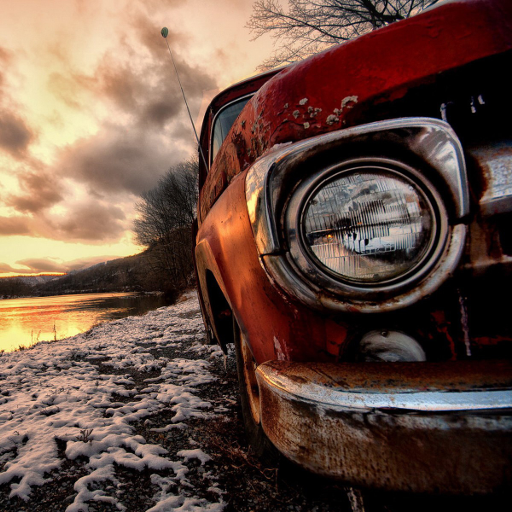
\includegraphics[width=7cm, height=6cm]{images/car.png}
        \caption{Original}
    \end{subfigure}%
    ~ 
    \begin{subfigure}[H]{0.5\textwidth}
        \centering
        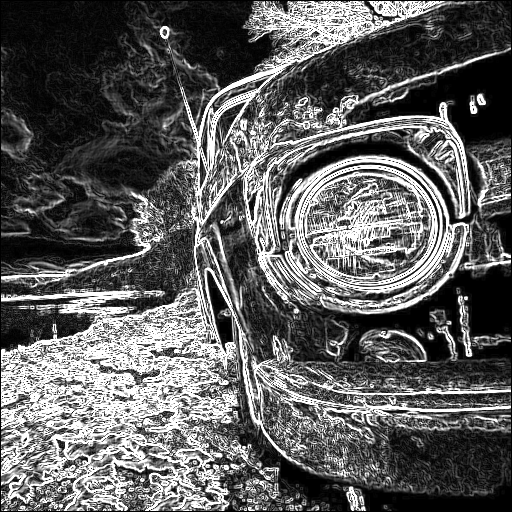
\includegraphics[width=7cm, height=6cm]{images/img_edgeSobel.png}
        \caption{Con Efecto Bayer}
    \end{subfigure}
    \caption{Caption place holder}
\end{figure} 

